%!TEX root = ../thesis.tex
\mychapter{Experimental Evaluation}{Experimental Evaluation}{}
\label{chap:evaluation}

This chapter reports what the pipeline did in two kinds of test. The virtual tests drive a simulated rover through a hand-drawn room map using typed commands, and they measure how long a chain of instructions can get before the plan stops matching the command (RQ2). The physical tests run the voice pipeline on the TurboPi in a real room, and they show which command levels in Table~\ref{tab:command-levels} the pipeline can carry out (RQ1). Every number below comes from the run logs produced by the pipeline itself, and the sample sizes are small enough that I report counts, not percentages.

\mysection{Experimental methodology}{Experimental Methodology}
\label{sec:methodology}

\mysubsection{Command corpus design}{Command Corpus Design}
\label{ssec:corpus}

\paragraph{Virtual tests.} The virtual rover moves through a hand-authored map of one room (\texttt{room\_tour1}), with every position expressed in a fixed metric frame and drift modelling switched off, so that any failure belongs to the plan and not to the simulated odometry. Commands are typed, and the audio loop is tested only on the physical rover. Four kinds of chain were generated, and each is scored against the sequence of landmarks the command asks for:
\begin{itemize}
  \item \emph{approach} chains of named landmarks (``go to the couch, then the coffee table, \ldots''), at depths of 1 to 12 instructions;
  \item \emph{literal} chains of metric moves and turns (``move forward 0.6 metres, turn right 90 degrees, \ldots''), at depths of 2 to 8;
  \item \emph{mixed} chains that combine the two, at depths of 4 to 8;
  \item \emph{probe} chains of depth 8 that contain one step the room or the rover cannot satisfy: a landmark that is not in the room, or an action outside the capability vocabulary (``pick up the lamp'').
\end{itemize}
Each command was run five times on the local pipeline and three times on the cloud benchmark. A separate context sweep (Section~\ref{sec:rq2_results}) used approach chains from depth 4 to 40 in steps of 4, three runs each, at three context settings.

\paragraph{Physical tests.} The physical tests use the command levels of Table~\ref{tab:command-levels}, with a level~0 control added in which the rover is only asked to describe what it sees. Each level has a small fixed set of commands built around two objects on the floor of the test room, an orange box and a black bag (later also a blue bottle). Commands are spoken, transcribed by the speech-to-text model, and confirmed by voice before the rover moves. The rover is never given a map or any marker, so every target has to be found by the camera.

\mysubsection{Evaluation metrics}{Evaluation Metrics}
\label{ssec:metrics}

For the virtual tests, a run counts as \emph{correct} when the plan visits exactly the expected landmarks in the expected order (\texttt{visits\_match}). A run is \emph{completed} when the mission reached the end of the plan, and \emph{halted} when the rover stopped on a blocked step. A \emph{hallucination} is an action, object or location in the plan that is not supported by the command, the room or the rover's capabilities, which is the definition used in Chapter~\ref{chap:introduction}. Collisions with virtual obstacles are counted separately.

For the physical tests, each run ends in one of four outcome classes recorded by the pipeline: \texttt{completed}, \texttt{completed\_after\_guidance} (the rover stopped, asked what to do next, and finished after the user answered), \texttt{halted\_after\_guidance}, and \texttt{aborted}. A run counts as handled when the logged plan matches the command and the rover reached its goal without intervention. I did not score the physical result of every run beyond the log, and Section~\ref{sec:rq1_results} marks where that matters.

\mysection{Plan correctness under vague commands}{Plan Correctness under Vague Commands}
\label{sec:rq1_results}

Table~\ref{tab:rq1_levels} summarises the final physical batch: 23 runs on the TurboPi with Gemma~4 E4B as both planner and vision model, recorded on 10 and 11 October.

\begin{table}[htbp]
    \centering
    \caption{Physical rover outcomes per command level, final batch (Gemma~4 E4B for planning and vision).}
    \label{tab:rq1_levels}
    \small
    \setlength{\tabcolsep}{5pt}
    \begin{tabular}{lp{3.6cm}rrrr}
        \toprule
        Level & Type & Runs & Done & After guid. & Halted/ aborted \\
        \midrule
        L0 & Describe scene (control) & 4 & 4 & 0 & 0 \\
        L1 & Single action & 3 & 3 & 0 & 0 \\
        L2 & Sequence of actions & 3 & 3 & 0 & 0 \\
        L3 & Perception-dependent & 4 & 1 & 2 & 1 \\
        L4 & Conditional & 7 & 6 & 0 & 1 \\
        L5 & Vague & 2 & 2 & 0 & 0 \\
        \midrule
        & Total & 23 & 19 & 2 & 2 \\
        \bottomrule
    \end{tabular}
\end{table}
\candidatetodo{L5 has only 2 runs; update this row and the total after the final two L5 runs, and add the raised-target (lamp on the desk) case.}

\paragraph{Levels 1 and 2.} All six runs produced the expected plan on the first attempt (\texttt{turn left, move forward} and \texttt{move forward, turn right, move forward}) and finished in 2 to 3\,s. These levels need no perception, so with three runs per level they show that the planner maps simple action chains onto the capability vocabulary without help, but they do not give a failure rate.

\paragraph{Level 3.} The plan shape was right in every run, because the pipeline turns ``drive forward until you see the black bag'' into an \texttt{approach} step followed by an \texttt{observe} and a \texttt{report}. Execution was less clean. Two of the four runs needed guidance (one needed three turns), and one halted after guidance. The halted run was the command ``please don't do the black bag'', which the pipeline resolved to ``drive to the black bag'' and then drove, so the negation was lost. The same batch contains transcripts that were visibly corrupted by the speech-to-text stage (``arif box'' for the orange box, ``go towards the orange box if you can see it and right to hear it''), and two of the four level~3 commands were of that kind. \candidatetodo{Check the spoken wording for these four runs; if ``don't'' was actually said, report it as a negation failure, otherwise as a transcription error.}

\paragraph{Level 4.} Five of the seven plans encoded the condition as an explicit \texttt{check} step followed by the branch (for example \texttt{check, approach, observe, report, stop}), and in those runs the rover either proceeded (three runs) or stayed put (two runs). Two plans dropped the condition entirely: the command was rewritten to ``go towards the orange box'' and the rover simply went. One of these two, with the black bag as the target, was aborted at an obstacle. Counting a dropped condition as a failure, five of seven level~4 plans were faithful to the command. \candidatetodo{Add whether each branch decision matched the true scene (box next to bottle or not) for each run; I cannot score this from the logs. Also drop or flag the run where the operator said where the box was.}

\paragraph{Level 5.} Both final-batch runs completed, but neither is a strong test of vagueness. One names the target outright (``tell me what is near the orange box''), and the other was a garbled command (``go towards the rn fox and then come to see a rally'') that the clarification loop turned into ``go to the orange box and tell me what you see around it''. The clarification step is what made this run work, which is the behaviour the design intends, but a single case cannot support a rate.

\paragraph{Exploratory runs.} Earlier runs between 7 and 9 October used different model pairs and are not part of Table~\ref{tab:rq1_levels}. In six search-and-approach runs with Gemma~4 E4B as the vision model, five halted after guidance with the target not found and one completed. In seven search-and-approach runs with Qwen2.5-VL~3B as the vision model, three completed directly, two completed after guidance, and two aborted. Six further runs on 9 October (levels 0 to 4, Qwen as the vision model) gave four direct completions, one completion after guidance and one halt after guidance. One of those completions is excluded because the spoken ``Thank you.'' was resolved to the previous command's plan, which shows that the dialogue state carried over between runs. These runs differ in command, planner and scene, so they are not a controlled comparison, and the final batch reached its targets with Gemma as the vision model, so the 8~October failures were not a permanent limit of that model. \candidatetodo{State what changed between 8 and 10 October (prompt, thresholds, scene), since the vision model alone does not explain the difference. Also say whether the dialogue state carry-over is fixed.}

\mysection{Executability on the physical chassis}{Executability on the Physical Chassis}
\label{sec:executability}

Because the rover has no wheel encoders and drives in short stop-look-hop cycles, two measurements decide whether a plan can be carried out safely: how well the ultrasonic sensor stops the rover, and whether the vision model can supply a distance estimate for the hop length.

\paragraph{Ultrasonic stop.} The stop threshold was set to 300\,mm. Table~\ref{tab:sonar} gives the sonar reading after the rover stopped. When the rover approached a box square-on or a wall, the reading after the stop was 184 to 291\,mm in all twelve runs, which is up to about 12\,cm inside the threshold because the sensor is polled at 100\,ms and two consecutive readings are required. The sonar did not see a box approached at 30\textdegree{} to the axis: it read 875 and 1097\,mm after the stop, so the beam passed beside the box. A thin chair leg stopped at 426\,mm. A low obstacle approached at an angle is therefore the case the ultrasonic layer does not cover, and the vision check is the only protection there.

\begin{table}[htbp]
    \centering
    \caption{Sonar reading after the rover stopped, per case (mm). Threshold 300\,mm.}
    \label{tab:sonar}
    \begin{tabular}{lcl}
        \toprule
        Case & Runs & Sonar after stop (mm) \\
        \midrule
        Box, square-on, from 50\,cm & 3 & 203, 231, 211 \\
        Box, square-on, from 30\,cm & 3 & 239, 291, 237 \\
        Box, square-on, from 20\,cm & 3 & 184, 203, 200 \\
        Wall & 3 & 206, 218, 206 \\
        Chair leg & 1 & 426 \\
        Box at 30\textdegree{} off-axis & 2 & 1097, 875 \\
        \bottomrule
    \end{tabular}
\end{table}
\candidatetodo{The sonar bench CSV stores the tape-measured gap in a column named gap\_cm, but the values (180 to 291) match the sonar readings in millimetres, so the recorded pass flags (15 of 15 against a 25\,cm limit) cannot be trusted. Confirm the units you typed, and recompute the pass count before citing it.}

\paragraph{Distance from vision.} Section~\ref{sec:rq1_results} relies on the vision model locating the target. I also tested whether it can report how far away the target is, using five true distances from 30 to 150\,cm with three frames each. The target was not visible in any frame at 30\,cm for the Gemma model and in all three for Qwen in numeric mode, because the camera is too low to see an object that close. For the other distances, Table~\ref{tab:f9} shows that neither model gave a usable absolute distance. Qwen2.5-VL~3B returned only two values (0.5\,m and 1.5\,m) in numeric mode, and in bucket mode it returned the same ``more than 2\,m'' bucket for every visible frame. Gemma~4 E4B tracked the ordering of the distances in numeric mode but overestimated by 1.25\,m on average, and in bucket mode its ranking was uncorrelated with the true distance. The variable hop length based on these estimates was therefore not adopted, and every mission in the final batch used the fixed hop.

\begin{table}[htbp]
    \centering
    \caption{Vision-model distance estimates against measured distance (visible frames only). MAE is the mean absolute error; the rank correlation is not defined for Qwen in bucket mode because its output was constant.}
    \label{tab:f9}
    \small
    \begin{tabular}{llrrr}
        \toprule
        Model & Mode & Frames & MAE (cm) & Rank corr. \\
        \midrule
        Gemma~4 E4B & numeric & 12 & 125 & 0.77 \\
        Gemma~4 E4B & bucket & 11 & 49 & $-0.12$ \\
        Qwen2.5-VL~3B & numeric & 12 & 40 & 0.43 \\
        Qwen2.5-VL~3B & bucket & 13 & 161 & n/a \\
        \bottomrule
    \end{tabular}
\end{table}

\mysection{Compositional depth and hallucination onset}{Compositional Depth and Hallucination Onset}
\label{sec:rq2_results}

Table~\ref{tab:rq2_depth} gives the virtual results for the local pipeline and the cloud benchmark. Across 105 local and 63 cloud chains of the approach, literal and mixed kinds, every plan visited the expected landmarks in the expected order. No hallucination was recorded in any of these 168 runs, so within the depths tested (up to 12 instructions for named landmarks and 8 for literal and mixed chains) I observed no onset of hallucination.

\begin{table}[htbp]
    \centering
    \caption{Virtual chains by kind and depth. Each cell gives correct plans and completed missions out of the runs (``Corr., compl.''), and the median planner latency in seconds (``Plan'').}
    \label{tab:rq2_depth}
    \small
    \setlength{\tabcolsep}{3pt}
    \begin{tabular}{llcccc}
        \toprule
        & & \multicolumn{2}{c}{Local (Gemma~4 E4B)} & \multicolumn{2}{c}{Cloud benchmark} \\
        \cmidrule(lr){3-4}\cmidrule(lr){5-6}
        Kind & Depth & Corr., compl. & Plan (s) & Corr., compl. & Plan (s) \\
        \midrule
        approach & 1 & 5/5, 5/5 & 1.0 & 3/3, 3/3 & 1.2 \\
        approach & 2 & 5/5, 5/5 & 1.2 & 3/3, 3/3 & 1.8 \\
        approach & 3 & 5/5, 5/5 & 4.0 & 3/3, 3/3 & 1.8 \\
        approach & 4 & 10/10, 10/10 & 4.2 & 6/6, 6/6 & 1.9 \\
        approach & 6 & 10/10, 10/10 & 2.5 & 6/6, 6/6 & 2.3 \\
        approach & 8 & 10/10, 10/10 & 2.7 & 6/6, 6/6 & 2.3 \\
        approach & 10 & 10/10, 10/10 & 6.0 & 6/6, 6/6 & 2.3 \\
        approach & 12 & 10/10, 10/10 & 4.7 & 6/6, 6/6 & 3.1 \\
        \midrule
        literal & 2 & 5/5, 5/5 & 1.4 & 3/3, 3/3 & 5.2 \\
        literal & 4 & 5/5, 5/5 & 1.9 & 3/3, 3/3 & 8.5 \\
        literal & 6 & 5/5, 5/5 & 3.4 & 3/3, 3/3 & 6.1 \\
        literal & 8 & 10/10, 10/10 & 3.1 & 6/6, 6/6 & 8.3 \\
        \midrule
        mixed & 4 & 5/5, 5/5 & 2.0 & 3/3, 3/3 & 7.1 \\
        mixed & 6 & 5/5, 5/5 & 5.6 & 3/3, 3/3 & 8.8 \\
        mixed & 8 & 5/5, 0/5 & 7.5 & 3/3, 2/3 & 12.3 \\
        \bottomrule
    \end{tabular}
\end{table}

\paragraph{Where execution failed.} The only non-completed non-probe runs are the depth-8 mixed chains, where the plan was correct but the mission halted. The command ``\ldots go to the bookshelf, turn left 90 degrees, move forward 0.6 metres, turn around, move forward 0.6 metres, \ldots'' produced a plan that followed the wording exactly, and the literal 0.6\,m move after the bookshelf collided with a virtual obstacle in five of five local runs and one of three cloud runs. The planner noted this risk itself (``the 0.6\,m straight movement \ldots may encounter an obstacle because \texttt{move} has no obstacle avoidance''). This is a plan that is faithful to the command but unsafe in the room, which is a different failure from hallucination and one that a literal command on a small rover will always allow.

\paragraph{Probe chains.} The probes test what the pipeline does when one step cannot be carried out. In all 9 cloud runs and 12 of the 15 local runs, the planner dropped the unresolvable step without saying so and returned a seven-step plan for an eight-step command, so the mission continued past the missing fridge or the unsupported ``pick up the lamp''. The remaining three local runs, all on the chain ending in the television, kept the step, and two of them halted on it, which is the intended behaviour. No unresolved target was logged for any of the nine cloud probes or the twelve silent local probes (\texttt{probe\_logged} false), and one local run was counted as a hallucination. The silent dropping of steps is the most important failure in the virtual tests, because it produces a plan that looks valid.

\paragraph{Context window and the plan ceiling.} Figure~\ref{fig:ctx} shows the context sweep. With the configured \texttt{num\_ctx} of 8192 the local planner produced correct plans for chains up to 36 instructions in all three runs, and at 40 instructions it produced a 34-step plan in all three runs, dropping the last six visits. The ceiling is therefore a plan-length limit of the model, and not a context limit, since it appears at 8192 where the plan uses only a fraction of the window.

\begin{figure}[htbp]
    \centering
    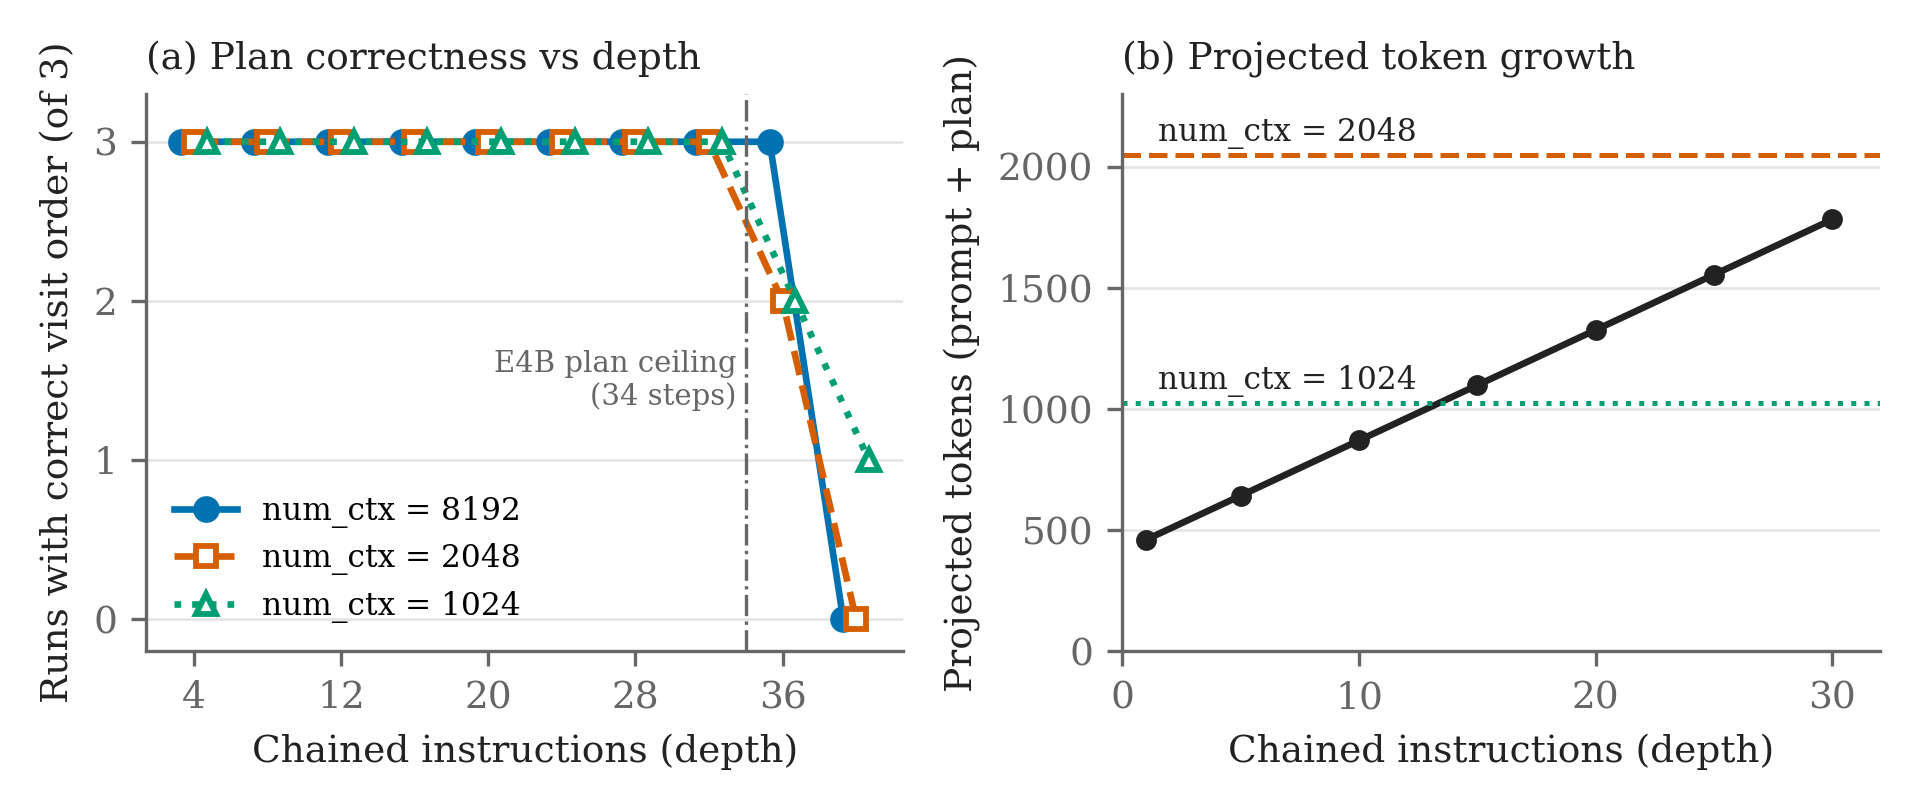
\includegraphics[width=\textwidth]{figures/fig_ctx_sweep.png}
    \caption{(a) Plans with the correct visit order out of three runs, against chain depth, at three context settings (points are offset horizontally for legibility). (b) Projected tokens per planning call against depth, measured to depth 30, with the 1024 and 2048 limits marked.}
    \label{fig:ctx}
\end{figure}

\begin{table}[htbp]
    \centering
    \caption{Correct plans out of three runs, by context setting and chain depth (Gemma~4 E4B).}
    \label{tab:ctx}
    \begin{tabular}{lcccc}
        \toprule
        \texttt{num\_ctx} & Depth 4--32 & 36 & 40 & Empty plans \\
        \midrule
        8192 & 3/3 at every depth & 3/3 & 0/3 (34 steps) & 0 \\
        2048 & 3/3 at every depth & 2/3 & 0/3 & 1 (depth 40) \\
        1024 & 3/3 at every depth & 2/3 & 1/3 & 1 (depth 40) \\
        \bottomrule
    \end{tabular}
\end{table}

Measuring the planning prompt gave 460 tokens at depth 1 and 1\,782 at depth 30 (about 46 tokens per added instruction), which is 22\% of the configured 8192-token window. For a mission that includes replanning with three guidance turns, the largest prompt measured was 1\,271 tokens at depth 30, and the largest revision prompt 1\,579 tokens. Extrapolating the single-shot slope gives an overflow at about depth 170 for 8192 tokens and about depth 2\,800 for the native 128K window, far beyond the 34-step ceiling. The same projection predicts overflow at about depth 13 for 1024 and about depth 36 for 2048 tokens. Table~\ref{tab:ctx} does not follow this for 1024: plans stayed correct up to depth 32 at a setting where the projection says the prompt should not fit. The prediction at 2048 matches the observed drop at depth 36 only by coincidence, since the same drop occurs at 8192. One empty plan at depth 40 appeared at each reduced setting and none at 8192, which is suggestive but is one run each. \candidatetodo{I could not verify that the server enforced the reduced context. Run ollama ps during a sweep (or an overflow probe longer than 1024 tokens) and state the loaded context length here before using the 1024 and 2048 results as evidence either way.}

\mysection{Reference comparison against cloud models}{Reference Comparison against Cloud Models}
\label{sec:cloud_comparison}

The cloud benchmark (gpt-5.6-luna through the OpenAI API) matched the local pipeline on plan correctness in every non-probe chain (63 of 63 against 105 of 105), and it behaved the same way on the probes, with the unresolvable step dropped silently in all nine runs. Across the non-probe chains the median planner latency was 3.1\,s for the local model and 2.6\,s for the cloud model, and the cloud model was slower on literal and mixed chains, where it needed 5 to 12\,s against 1.4 to 7.5\,s locally (Table~\ref{tab:rq2_depth}). In these tests the cloud model had no advantage in correctness and none in latency, which is consistent with the project's premise that a small local model is enough for the plan-generation step. Two limits apply. The cloud runs stop at depth 12 for named landmarks and did not include the depth-40 sweep, so the 34-step ceiling cannot be compared, and no cloud run was made on the physical rover.

\mysection{Discussion}{Discussion}
\label{sec:discussion}

\paragraph{RQ1.} On the physical rover, the local pipeline handled levels 0 to 2 without help in all ten runs, and levels 3 to 5 ended in a completed mission in 11 of 13 runs (nine directly and two after guidance), with one run halted after guidance at level~3 and one aborted at level~4. Its main weakness at level~4 was dropping the condition in two of seven plans, and its main weakness at level~3 was speech-to-text noise, which twice changed or lost the meaning of the command. Reliability at levels 3 to 5 is therefore supported by a handful of runs and should be reported as a demonstration of capability, not as a rate. The part of the design that earns its place is the guidance loop, which turned several runs that would have ended with ``target not found'' into completed missions.

\paragraph{RQ2.} In the virtual tests no hallucinated step appeared in chains of up to 12 named landmarks or 8 literal instructions, and chains of up to 36 instructions stayed correct at the configured context. The first failure mode is not hallucination but truncation, at about 34 steps, followed by the silent dropping of steps that cannot be carried out. Neither failure is caught by the pipeline at plan time, which argues for a capability check on the plan before departure as the most useful next improvement.

\paragraph{Limitations.} The evidence is one room, one rover, and three to seven runs per physical level. Level~5 is not yet adequately covered, the level~4 branches have not been scored against the true scene, and the vision-based distance estimate was not good enough to use. The virtual tests switch odometry drift off and use typed text, so they separate plan quality from perception and speech, and they are not directly comparable to the physical runs. The ultrasonic stop does not protect against low obstacles approached at an angle.
